\documentclass{standalone}

\usepackage{tikz}
\usetikzlibrary{arrows}
\usetikzlibrary{arrows.meta}
\usetikzlibrary{decorations.markings}
\usepackage{pgfplots}

\tikzset{>={Latex[length=3mm]}}

\begin{document}
\pagestyle{empty}
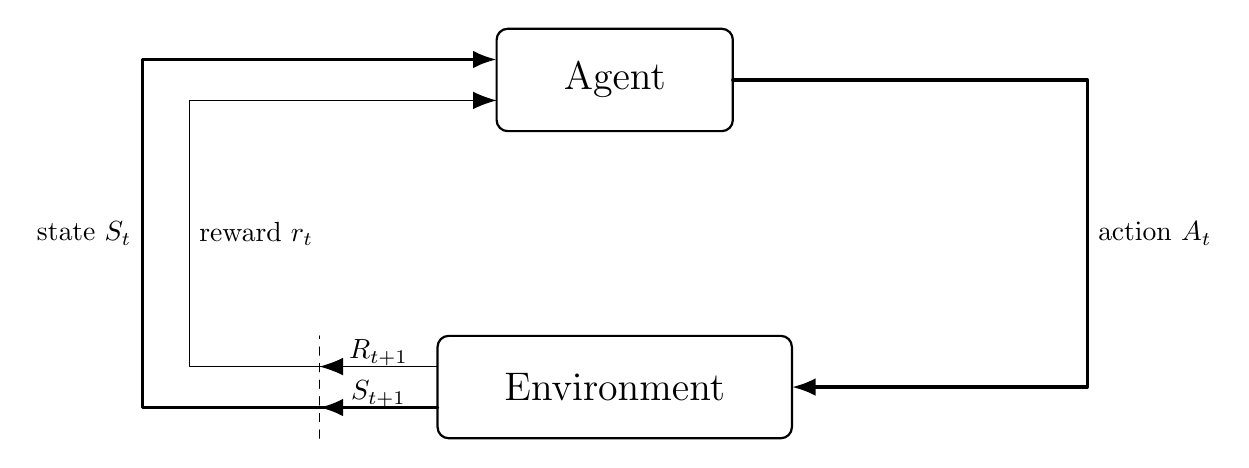
\begin{tikzpicture}[xscale=1.5, yscale=1.3, line cap=round,line join=round]

\draw[rounded corners, thick] (0.5,0) rectangle(3.5,1) node[midway] {\Large Environment\normalsize};

\draw[rounded corners, thick] (1,3) rectangle(3,4) node[midway] {\Large Agent \normalsize};
 
\draw[->, very thick] (0.5,0.3) -- (-2,0.3) --node[left,midway]{state $S_t$} (-2,3.7) -- (1,3.7);
\draw[->] (0.5,0.7) -- (-1.6,0.7) --node[right,midway]{reward $r_t$} (-1.6,3.3) -- (1,3.3);

\draw[->, very thick] (3,3.5) -- (6,3.5) --node[right, midway]{action $A_t$} (6,0.5) -- (3.5,0.5);

\draw[-, dashed] (-0.5,0) -- (-0.5,1);
\draw[->] (0.5,0.7) -- (-0.5,0.7) node[midway,yshift=5]{$R_{t+1}$};
\draw[->, very thick] (0.5,0.3) -- (-0.5,0.3) node[midway, yshift=5]{$S_{t+1}$};

\end{tikzpicture}

\end{document}